\documentclass[11pt,a4paper]{article}

% --- Encodage & langue ---
\usepackage[utf8]{inputenc}
\usepackage[T1]{fontenc}
\usepackage[french]{babel}
\usepackage{lmodern}

% --- Mise en page ---
\usepackage[margin=2.5cm]{geometry}
\usepackage{microtype}
\usepackage{parskip}
\usepackage{setspace}
\usepackage{fancyhdr}
\linespread{1.06}

% --- Maths, tableaux, figures, code ---
\usepackage{amsmath}
\usepackage{booktabs}
\usepackage{array}
\usepackage{graphicx}
\usepackage{float}
\usepackage{xcolor}
\usepackage{listings}

% --- Liens ---
\usepackage[hidelinks]{hyperref}
\hypersetup{
  colorlinks=true, linkcolor=black, urlcolor=blue!60!black, citecolor=black,
  pdftitle={Naive Bayes multinomial en MapReduce sur Spark},
  pdfauthor={Abdrahamane Mbourou Camara},
  pdfsubject={ML on Big Data - Master MIAGE SITN, Universite Paris-Dauphine},
  pdfkeywords={Naive Bayes, MapReduce, Apache Spark, RDD, DataFrames, scalabilite}
}

% --- Palette ------------------------------------------------------------------
\definecolor{primary}{RGB}{23,54,101}   % bleu nuit (titres, filets)
\definecolor{accent}{RGB}{176,58,46}    % rouge sobre (accents)
\definecolor{codebg}{gray}{0.96}
\definecolor{outbg}{rgb}{0.94,0.96,1.0}
\definecolor{kw}{rgb}{0.0,0.2,0.7}
\definecolor{cmt}{rgb}{0.30,0.55,0.30}
\definecolor{str}{rgb}{0.6,0.1,0.1}

% Table de correspondance Unicode -> LaTeX pour inclure le code source verbatim.
\lstset{
  inputencoding=utf8,
  extendedchars=true,
  literate=%
    {é}{{\'e}}1 {è}{{\`e}}1 {à}{{\`a}}1 {ê}{{\^e}}1 {î}{{\^i}}1 {ô}{{\^o}}1
    {â}{{\^a}}1 {û}{{\^u}}1 {ù}{{\`u}}1 {ç}{{\c c}}1 {ï}{{\"i}}1 {ë}{{\"e}}1
    {ü}{{\"u}}1 {ö}{{\"o}}1 {É}{{\'E}}1 {È}{{\`E}}1 {Ê}{{\^E}}1 {À}{{\`A}}1
    {Ç}{{\c C}}1 {œ}{{\oe}}1 {Œ}{{\OE}}1 {«}{{\guillemotleft}}1
    {»}{{\guillemotright}}1 {—}{{---}}1 {–}{{--}}1 {±}{{$\pm$}}1
    {≈}{{$\approx$}}1 {×}{{$\times$}}1 {→}{{$\rightarrow$}}1 {✅}{{[OK]}}1
    {❌}{{[X]}}1 {⚠}{{[!]}}1 {…}{{...}}1 {✓}{{v}}1
    {Î}{{\^I}}1 {Ï}{{\"I}}1 {Ô}{{\^O}}1 {Â}{{\^A}}1 {Û}{{\^U}}1 {Ù}{{\`U}}1
    {Ë}{{\"E}}1 {Ü}{{\"U}}1 {Ö}{{\"O}}1 {§}{{\S}}1 {·}{{\textperiodcentered}}1
    {°}{{\textdegree}}1 {α}{{$\alpha$}}1 {β}{{$\beta$}}1 {≠}{{$\neq$}}1
    {≤}{{$\leq$}}1 {≥}{{$\geq$}}1 {∑}{{$\sum$}}1
}

\lstdefinestyle{py}{
  language=Python,
  basicstyle=\ttfamily\footnotesize,
  keywordstyle=\color{kw}\bfseries,
  commentstyle=\color{cmt}\itshape,
  stringstyle=\color{str},
  backgroundcolor=\color{codebg},
  frame=single, framerule=0pt, framesep=4pt,
  breaklines=true, breakatwhitespace=false,
  columns=fullflexible, keepspaces=true, showstringspaces=false,
  numbers=none, aboveskip=1ex, belowskip=1ex,
}
\lstdefinestyle{nboutput}{
  basicstyle=\ttfamily\footnotesize,
  backgroundcolor=\color{outbg},
  frame=single, framerule=0pt, framesep=4pt,
  breaklines=true, columns=fullflexible, keepspaces=true,
}
\lstset{style=py}   % style par défaut
\newcommand{\code}[1]{\lstinline[style=py]!#1!}

% --- Titres de sections colorés (sans titlesec, indisponible) -----------------
\makeatletter
\renewcommand\section{\@startsection{section}{1}{\z@}%
  {-3.5ex \@plus -1ex \@minus -.2ex}{2.2ex \@plus.2ex}%
  {\normalfont\Large\bfseries\color{primary}}}
\renewcommand\subsection{\@startsection{subsection}{2}{\z@}%
  {-3.0ex \@plus -1ex \@minus -.2ex}{1.3ex \@plus.2ex}%
  {\normalfont\large\bfseries\color{primary!88!black}}}
\renewcommand\subsubsection{\@startsection{subsubsection}{3}{\z@}%
  {-2.8ex \@plus -1ex \@minus -.2ex}{1.1ex \@plus.2ex}%
  {\normalfont\normalsize\bfseries\color{primary!72!black}}}
\makeatother

% --- En-têtes / pieds de page -------------------------------------------------
\pagestyle{fancy}
\fancyhf{}
\fancyhead[L]{\small\itshape Naive Bayes en MapReduce sur Spark}
\fancyhead[R]{\small\thepage}
\renewcommand{\headrulewidth}{0.4pt}
\renewcommand{\footrulewidth}{0pt}
\setlength{\headheight}{14pt}

\begin{document}

% ============================== PAGE DE TITRE =================================
\thispagestyle{empty}
\vspace*{2.2cm}
\begin{center}
{\color{primary}\rule{\linewidth}{1.6pt}}\\[0.8cm]
{\Huge\bfseries\color{primary} ML on Big Data\par}
\vspace{0.5cm}
{\LARGE Naive Bayes multinomial\\[0.2em] en MapReduce sur Spark\par}
\vspace{0.5cm}
{\large\itshape K-NN \emph{or} Naive Bayes --- option Naive Bayes\par}
\vspace{0.7cm}
{\color{primary}\rule{\linewidth}{1.6pt}}\\[1.8cm]
{\Large\bfseries Abdrahamane MBOUROU CAMARA\par}
\vspace{0.6cm}
{\large Master MIAGE SITN\\[0.2em] Université Paris-Dauphine\par}
\vspace{0.5cm}
{\large Cours « ML on Big Data » --- Prof. D. Colazzo\par}
\end{center}
\vfill
\begin{center}{\large Juillet 2026}\end{center}
\clearpage

% ============================== TABLE DES MATIÈRES ============================
\begingroup
\setlength{\parskip}{0.35em}
\tableofcontents
\endgroup
\clearpage

% ============================== GUIDE DE LECTURE =============================
\section*{Organisation du rapport et correspondance avec le barème}
Ce document est structuré pour répondre \emph{explicitement}, section par section, aux
cinq items notés de l'énoncé (total 20 points).

\begin{table}[H]
\centering
\small
\renewcommand{\arraystretch}{1.25}
\begin{tabular}{@{}p{8.6cm}cc@{}}
\toprule
\textbf{Item du barème} & \textbf{Points} & \textbf{Section} \\
\midrule
1. Description de la solution adoptée & 3 & \S\ref{sec:solution} \\
2a. Algorithmes conçus + description globale & 3 & \S\ref{sec:algos} \\
2b. Commentaires des fragments de code clés & 3 & \S\ref{sec:fragments} \\
3. Analyse expérimentale (scalabilité) & 3 & \S\ref{sec:scalability} \\
4. Points forts / points faibles des algorithmes & 3 & \S\ref{sec:forces} \\
5. Annexe : tout le code + notebook (petites données, E/S commentées) & 4 & Annexes \ref{sec:annexe-code}--\ref{sec:annexe-nb} \\
\bottomrule
\end{tabular}
\end{table}
\vspace{0.4em}

% ==============================================================================
\section{Description de la solution adoptée \hfill\normalsize\textmd{[Item 1 --- 3 pts]}}
\label{sec:solution}

\subsection{Problème}
On implémente le classifieur \textbf{Naive Bayes} selon le paradigme \textbf{MapReduce}
sur Apache Spark, en s'appuyant sur l'algorithme du papier de référence~\cite{nbmapreduce}
(Zheng, NDSU, 2014). Le classifieur est codé en \textbf{deux versions} (contrainte de
l'énoncé), \textbf{en Python uniquement} :
\begin{itemize}
  \item version \textbf{RDD} (API bas niveau : \code{map} / \code{reduceByKey}) ;
  \item version \textbf{DataFrames} (API relationnelle : \code{explode} + \code{groupBy}/\code{agg}).
\end{itemize}
Exigence forte que nous garantissons : les deux versions produisent des \textbf{prédictions
rigoureusement identiques} (\S\ref{sec:identite}).

Nous couvrons \textbf{deux lois} partageant exactement le même cœur MapReduce (seul le calcul
du modèle diffère, \S\ref{sec:categorical}) :
\begin{itemize}
  \item \textbf{multinomial} pour la classification de \emph{texte} (sac de mots) ;
  \item \textbf{catégoriel} pour les jeux \emph{tabulaires} du papier (attribut-valeur),
        avec discrétisation des attributs continus.
\end{itemize}

\subsection{Données}
\begin{table}[H]
\centering\small
\begin{tabular}{@{}llll@{}}
\toprule
\textbf{Jeu} & \textbf{Rôle} & \textbf{Taille} & \textbf{Source} \\
\midrule
SMS Spam Collection & démo texte / smoke test (petit) & 5\,574 SMS (ham/spam) & UCI \\
20 Newsgroups & scalabilité (grand) & 18\,846 docs, 20 classes & scikit-learn \\
mushroom, car, nursery, adult & variante catégorielle (papier) & 1\,7k--32k instances & UCI \\
\bottomrule
\end{tabular}
\end{table}
Les jeux tabulaires sont exactement ceux du papier de référence, ce qui permet une
comparaison directe (\S\ref{sec:comparaison}). L'énoncé autorise « datasets of your choice ».
Le petit jeu sert au notebook et au smoke test ; le grand jeu sert à l'étude de scalabilité.
Pour 20 Newsgroups, en-têtes, pieds de page et citations sont retirés pour ne garder qu'un
signal textuel.

\subsection{Architecture logicielle}
La solution isole dans un module \textbf{commun} (\code{src/nb_common.py}) tout ce qui doit
être identique entre les deux versions : tokenisation, vocabulaire, découpage,
\emph{construction du modèle} (comptes $\to$ log-probabilités) et \emph{fonction de
prédiction}. Les modules \code{src/nb_rdd.py} et \code{src/nb_dataframe.py} ne font que
produire, chacun à sa manière (map/reduce), les mêmes \emph{comptes entiers}, puis délèguent
au module commun. C'est ce qui rend l'égalité des prédictions vraie \emph{par construction}.

\begin{table}[H]
\centering\small
\begin{tabular}{@{}ll@{}}
\toprule
\textbf{Fichier} & \textbf{Rôle} \\
\midrule
\code{src/nb_common.py}    & tokenisation, vocabulaire, split, \code{build_model}, \code{predict_indices}, \code{get_spark} \\
\code{src/nb_rdd.py}       & entraînement/prédiction en RDD (\code{flatMap}/\code{reduceByKey} + broadcast) \\
\code{src/nb_dataframe.py} & idem en DataFrames (\code{explode} + \code{groupBy}/\code{agg} + UDF) \\
\code{src/benchmark.py}    & étude de scalabilité $\to$ \code{results.csv} + graphes PNG \\
\code{data/download\_*.py}  & récupération SMS Spam / 20 Newsgroups \\
\code{tests/test\_smoke.py} & test d'égalité RDD == DataFrame \\
\code{notebooks/demo.ipynb} & démo end-to-end sur petites données + comparaison sklearn \\
\bottomrule
\end{tabular}
\end{table}

% ==============================================================================
\section{Algorithmes conçus et description globale \hfill\normalsize\textmd{[Item 2a --- 3 pts]}}
\label{sec:algos}

\subsection{Le modèle Naive Bayes multinomial}
Pour un document $d$, une classe $c$, un vocabulaire de taille $V$ et un lissage de Laplace
$\alpha=1$, tous les calculs se font \textbf{en logarithme} (pour éviter les
sous-débordements numériques) :
\begin{align}
  \log P(c)      &= \log\!\left( \frac{N_c}{N} \right), &
  \log P(w \mid c) &= \log\!\left( \frac{\mathrm{count}_{w,c} + \alpha}{\mathrm{total}_c + \alpha V} \right),
\end{align}
avec $N$ le nombre de documents d'entraînement, $N_c$ ceux de la classe $c$,
$\mathrm{count}_{w,c}$ les occurrences du mot $w$ en classe $c$, et
$\mathrm{total}_c=\sum_w \mathrm{count}_{w,c}$. La prédiction maximise :
\begin{equation}
  \mathrm{score}(d,c) = \log P(c) + \sum_{w\in d}\mathrm{count}_w(d)\,\log P(w\mid c).
\end{equation}
Le modèle reproduit exactement \code{sklearn.naive\_bayes.MultinomialNB} ($\alpha=1$,
\code{fit\_prior=True}), ce qui est vérifié empiriquement (\S\ref{sec:identite}).

\subsection{Formulation MapReduce (entraînement)}
L'entraînement se ramène à des \textbf{comptages} --- cas idéal pour MapReduce. Le cœur est
$\mathrm{count}_{w,c}$ :
\begin{itemize}
  \item \textbf{MAP} : pour chaque occurrence d'un mot $w$ dans un document de classe $c$,
        émettre la paire $\big((c,w),\,1\big)$.
  \item \textbf{REDUCE} : sommer les $1$ par clé $(c,w)$ $\to \mathrm{count}_{w,c}$.
\end{itemize}
On compte de même $N_c$ (documents par classe) et $\mathrm{total}_c$ (tokens par classe).
La version RDD exprime le MAP par \code{flatMap} et le REDUCE par \code{reduceByKey} ; la
version DataFrames exprime le MAP par \code{explode} (une ligne par mot) et le REDUCE par
\code{groupBy(label, word).count()}.

\subsection{Construction du modèle et broadcast}
Les deux versions passent les mêmes \emph{comptes entiers} à la fonction commune
\code{build\_model}, qui calcule les log-probabilités lissées. Le modèle est stocké de façon
\textbf{creuse mais équivalente au dense} : $\log P(w\mid c)$ n'est mémorisé que pour les
$(c,w)$ de compte non nul, plus une valeur par défaut
$\log(\alpha/(\mathrm{total}_c+\alpha V))$ pour les mots de compte nul. Ce modèle est
\textbf{broadcasté} (\code{sc.broadcast}) : Spark l'envoie une fois par worker (lecture
seule) au lieu de le re-sérialiser à chaque tâche.

\subsection{Garantie de prédictions identiques}
\label{sec:identite}
Les comptes étant entiers (reproductibles au bit près) et la prédiction déterministe (même
fonction \code{predict\_indices}), les deux versions donnent des prédictions identiques
\emph{par construction}. \textbf{Vérifications} : le smoke test impose
l'égalité RDD/DataFrame ; le notebook obtient \textbf{accuracy $=0.9848$} sur SMS Spam avec
\textbf{RDD $=$ DataFrame $=$ sklearn} (prédictions identiques) ; le benchmark \code{assert}
l'égalité des accuracy sur chacun des 16 points de mesure.

\subsection{Variante catégorielle (jeux tabulaires du papier)}
\label{sec:categorical}
Le papier applique en réalité Naive Bayes à des données \emph{tabulaires catégorielles}.
Chaque instance a $M$ attributs ; on estime, pour un attribut $A_i$ de valeur $a$ :
\begin{equation}
  \log P(A_i = a \mid c) = \log\!\left( \frac{\mathrm{count}_{a,i,c} + \alpha}{N_c + \alpha D_i} \right),
\end{equation}
où $D_i$ est la taille du domaine de l'attribut $i$. La \textbf{seule différence} avec le
multinomial est le \emph{dénominateur} ($N_c$, nombre d'instances de la classe, au lieu du
total de tokens). Le \textbf{comptage MapReduce est identique} : on encode chaque instance
comme un sac de features (attribut, valeur), on émet $\big((c, \text{feature}), 1\big)$ et on
somme. Seul le calcul du modèle change : dans le code, on branche
\code{build\_model\_categorical} via le paramètre \code{model\_builder} des fonctions
d'entraînement --- la prédiction reste \code{predict\_indices}, donc RDD $=$ DataFrame reste
vrai. Ce modèle reproduit \code{sklearn.naive\_bayes.CategoricalNB} (vérifié).

Les attributs \textbf{continus} (jeu \emph{adult}) sont d'abord \textbf{discrétisés} : un
premier job MAP/REDUCE calcule (min, max) par colonne (comme le \emph{PreprocessMapper} du
papier), puis on découpe en tranches (binning). C'est la structure à \textbf{deux jobs
MapReduce} du papier.

% ==============================================================================
\section{Commentaires des fragments de code clés \hfill\normalsize\textmd{[Item 2b --- 3 pts]}}
\label{sec:fragments}

\subsection{Cœur MapReduce, version RDD (\texttt{src/nb\_rdd.py})}
Le MAP émet une paire par occurrence de mot ; le REDUCE (\code{reduceByKey}) somme.
\begin{lstlisting}[style=py]
# MAP : pour un doc (c, [w1, w2, w1, ...]) on émet ((c, w1), 1), ((c, w2), 1), ...
def emit_word_class(doc):
    c, word_indices = doc
    for w in word_indices:
        yield ((c, w), 1)          # une paire clé/valeur par occurrence

# REDUCE : reduceByKey(add) additionne toutes les occurrences -> count_{w,c}
word_class_counts = dict(
    docs.flatMap(emit_word_class).reduceByKey(add).collect()
)
\end{lstlisting}

\subsection{Cœur MapReduce, version DataFrames (\texttt{src/nb\_dataframe.py})}
\code{explode} joue le rôle du MAP (une ligne par mot) ; \code{groupBy().count()} celui du
REDUCE.
\begin{lstlisting}[style=py]
# MAP  : explode(words) -> une ligne (label, word) PAR occurrence de mot
exploded = df.select("label", F.explode("words").alias("word"))
# REDUCE : groupBy(label, word).count() -> count_{w,c}
word_class_counts = {
    (r["label"], r["word"]): r["cnt"]
    for r in exploded.groupBy("label", "word").agg(F.count("*").alias("cnt")).collect()
}
\end{lstlisting}

\subsection{Calcul du modèle (\texttt{src/nb\_common.py})}
Passage des comptes entiers aux log-probabilités, avec lissage de Laplace ; factorisé pour
être \emph{identique} dans les deux versions.
\begin{lstlisting}[style=py]
# Dénominateur commun à une classe : total_c + alpha * V
denom = [class_token_totals.get(c, 0) + alpha * vocab_size for c in range(n_classes)]
# Valeur par défaut (mot de compte nul dans la classe) : log(alpha / denom)
log_likelihood_default = [math.log(alpha / denom[c]) for c in range(n_classes)]
# Pour chaque (classe, mot) observé : log((count + alpha) / denom)
for (c, w), count in word_class_counts.items():
    log_likelihood[c][w] = math.log((count + alpha) / denom[c])
# Priors : log P(c) = log(N_c / N)
log_prior[c] = math.log(class_doc_counts[c] / n_docs)
\end{lstlisting}

\subsection{Broadcast du modèle et prédiction}
Le modèle est diffusé une fois par worker, puis utilisé en lecture seule (map RDD / UDF DF).
\begin{lstlisting}[style=py]
# --- RDD ---
bc_model = sc.broadcast(model)                 # diffusion en lecture seule
preds = docs.map(lambda cw: C.predict_indices(bc_model.value, cw[1])).collect()

# --- DataFrame ---
bc_model = sc.broadcast(model)
@F.udf(returnType=IntegerType())
def predict_udf(words):                        # closure référençant bc_model.value
    return int(C.predict_indices(bc_model.value, words or []))
\end{lstlisting}
\emph{Remarque technique} : \code{get\_spark()} appelle \code{sc.addPyFile(...)} sur nos
modules, sans quoi les workers lèveraient \code{ModuleNotFoundError: nb\_common} lors de la
désérialisation du modèle et de l'appel à \code{predict\_indices}.

\subsection{Modèle catégoriel et discrétisation (variante du papier)}
Même comptage, dénominateur différent ($N_c + \alpha D_i$) ; et le job de discrétisation
(min/max) est un MAP/REDUCE à part entière.
\begin{lstlisting}[style=py]
# Modèle CATÉGORIEL : denom dépend de l'attribut de la feature (N_c + alpha * D_i)
for c in range(n_classes):
    n_c = class_doc_counts.get(c, 0)
    for f in range(vocab_size):
        d_i = attr_domain_sizes[feature_attr[f]]        # taille du domaine de l'attribut
        cnt = word_class_counts.get((c, f), 0)
        log_likelihood[c][f] = math.log((cnt + alpha) / (n_c + alpha * d_i))

# Discrétisation : 1er job MAP/REDUCE calculant (min, max) par colonne continue
def emit(row):
    for col in continuous_cols:
        yield (col, (float(row[col]), float(row[col])))          # MAP
minmax = sc.parallelize(rows).flatMap(emit) \
           .reduceByKey(lambda a, b: (min(a[0], b[0]), max(a[1], b[1]))).collect()  # REDUCE
\end{lstlisting}

% ==============================================================================
\section{Analyse expérimentale : scalabilité \hfill\normalsize\textmd{[Item 3 --- 3 pts]}}
\label{sec:scalability}

\subsection{Protocole}
\begin{itemize}
  \item \textbf{Machine} : macOS (Apple Silicon, arm64), 8 cœurs (4 \emph{performance} + 4
        \emph{efficiency}). Spark en mode local (\code{local[k]}).
  \item \textbf{Expérience A --- volume} : à \code{local[*]}, réplication de 20 Newsgroups par
        un facteur $\in\{{\times}1,{\times}2,{\times}4,{\times}8\}$.
  \item \textbf{Expérience B --- parallélisme} : à volume fixe (${\times}8$, $\sim$121\,k docs),
        variation de \code{local[k]}, $k\in\{1,2,4,8\}$.
  \item \textbf{Anti-fuite} : la réplication est faite \textbf{après} le découpage train/test,
        séparément de chaque côté (un document de test ne peut jamais apparaître, même
        dupliqué, dans l'entraînement).
  \item \textbf{Bruit de mesure} : \code{--repeat 3} --- chaque point mesuré 3 fois, agrégé en
        moyenne $\pm$ écart-type (barres d'erreur sur les figures).
\end{itemize}
Commande : \code{python src/benchmark.py --factors 1 2 4 8 --cores 1 2 4 8 --repeat 3}.

\subsection{Résultats --- scalabilité en volume}
\begin{table}[H]
\centering\small
\begin{tabular}{@{}rrrrrrr@{}}
\toprule
\textbf{Facteur} & \textbf{n\_train} & \textbf{RDD train} & \textbf{DF train} & \textbf{RDD pred} & \textbf{DF pred} & \textbf{Acc.} \\
\midrule
${\times}1$ & 15\,076  & $1.81\pm0.67$ & $3.07\pm1.25$ & $0.44\pm0.04$ & $1.39\pm0.27$ & 0.620 \\
${\times}2$ & 30\,152  & $1.89\pm0.15$ & $3.10\pm0.20$ & $0.68\pm0.04$ & $2.01\pm0.19$ & 0.677 \\
${\times}4$ & 60\,304  & $3.16\pm0.15$ & $5.11\pm0.25$ & $1.26\pm0.03$ & $3.42\pm0.21$ & 0.704 \\
${\times}8$ & 120\,608 & $5.27\pm0.11$ & $8.57\pm0.09$ & $2.29\pm0.09$ & $6.91\pm1.10$ & 0.711 \\
\bottomrule
\end{tabular}
\caption{Temps (s, moyenne $\pm$ écart-type sur 3 exécutions) selon le volume, à \code{local[*]}.}
\end{table}
\begin{figure}[H]\centering
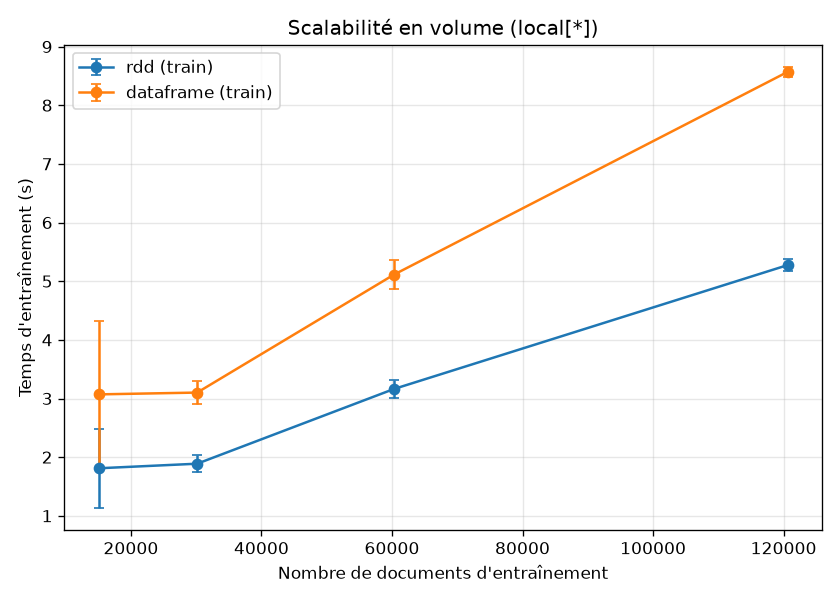
\includegraphics[width=0.72\linewidth]{figures/scalability_datasize.png}
\caption{Temps d'entraînement en fonction du volume (\code{local[*]}).}
\end{figure}
De ${\times}1$ à ${\times}8$ (8$\times$ de données), le temps d'entraînement ne croît que
d'un facteur ${\sim}2.9$ : \textbf{passage à l'échelle sous-linéaire}. RDD est plus rapide que
DataFrames à tous les points ; la prédiction DataFrames est ${\sim}3\times$ plus lente
(UDF Python ligne à ligne).

\subsection{Résultats --- scalabilité en parallélisme}
\begin{table}[H]
\centering\small
\begin{tabular}{@{}rrrrrr@{}}
\toprule
\textbf{Cœurs} & \textbf{RDD train} & \textbf{speed-up} & \textbf{RDD pred} & \textbf{DF train} & \textbf{DF pred} \\
\midrule
1 & $12.66\pm0.30$ & $1.00\times$ & $5.00\pm0.04$ & $10.05\pm0.07$ & $12.07\pm0.36$ \\
2 & $7.23\pm0.15$  & $1.75\times$ & $3.34\pm0.08$ & $9.13\pm0.30$  & $8.63\pm0.02$ \\
4 & $5.88\pm0.57$  & $\mathbf{2.15\times}$ & $2.68\pm0.28$ & $9.18\pm0.27$  & $8.09\pm0.53$ \\
8 & $10.97\pm1.51$ & $1.15\times$ & $3.48\pm0.51$ & $12.55\pm1.45$ & $8.30\pm0.85$ \\
\bottomrule
\end{tabular}
\caption{Temps (s) selon le nombre de cœurs, à volume fixe (${\times}8$). Speed-up $=T(1)/T(k)$.}
\end{table}
\begin{figure}[H]\centering
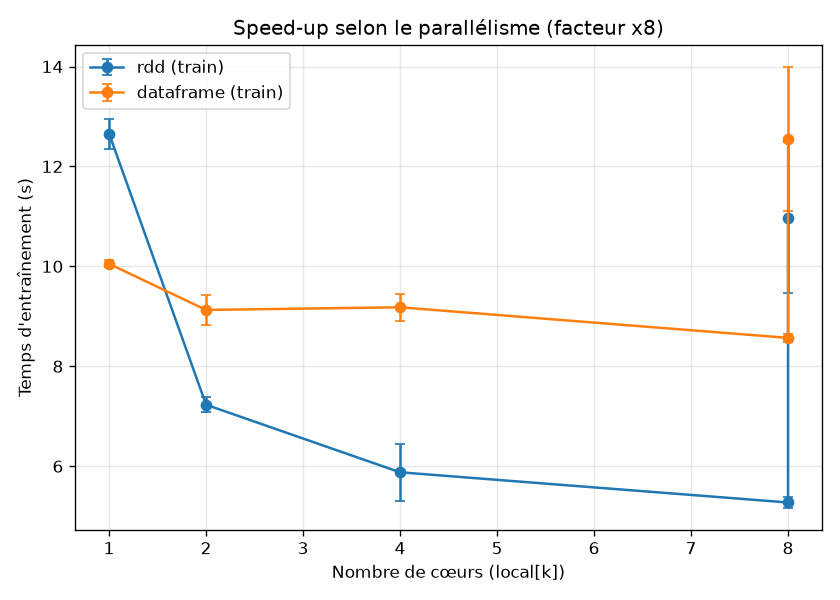
\includegraphics[width=0.72\linewidth]{figures/scalability_cores.png}
\caption{Temps d'entraînement en fonction du nombre de cœurs (facteur ${\times}8$).}
\end{figure}
Le speed-up RDD progresse jusqu'à ${\sim}2.15\times$ à 4 cœurs, puis \textbf{régresse à 8
cœurs} : sur Apple Silicon, \code{local[8]} embarque les 4 cœurs \emph{efficiency} (plus
lents) et met le driver en contention, d'où un point plus lent et fortement bruité
($\pm1.5$\,s). DataFrames ne profite quasiment pas des cœurs supplémentaires.

\subsection{Évaluation détaillée : validation croisée et métriques}
\label{sec:cv}
Au-delà de l'accuracy sur un seul découpage, on suit la méthodologie du papier (§2.3.3--2.3.4) :
\textbf{validation croisée k-fold} et métriques \textbf{précision / rappel / F1} + matrice de
confusion. Sur SMS Spam (multinomial), en 5-fold : \textbf{accuracy $= 0.9865 \pm 0.0029$}.
La matrice de confusion et les métriques par classe (obtenues dans le notebook) :
\begin{table}[H]
\centering\small
\begin{tabular}{@{}lrrr@{}}
\toprule
\textbf{Classe} & \textbf{Précision} & \textbf{Rappel} & \textbf{F1} \\
\midrule
ham  & 0.986 & 0.997 & 0.991 \\
spam & 0.978 & 0.906 & 0.941 \\
\midrule
\textbf{macro} & 0.982 & 0.951 & \textbf{0.966} \\
\bottomrule
\end{tabular}
\caption{Métriques par classe sur SMS Spam (holdout 80/20). Le rappel plus faible du
\emph{spam} (0.906) révèle ce que l'accuracy globale (0.985) masque.}
\end{table}

\subsection{Variante catégorielle sur les jeux UCI du papier}
\label{sec:uci}
On applique le \textbf{Naive Bayes catégoriel} (avec discrétisation pour \emph{adult}) sur les
quatre jeux tabulaires du papier, en \textbf{6-fold CV}. À chaque pli, RDD $=$ DataFrames
(vérifié par \code{assert}).
\begin{table}[H]
\centering\small
\begin{tabular}{@{}lrrrrr@{}}
\toprule
\textbf{Jeu} & \textbf{Instances} & \textbf{Classes} & \textbf{Accuracy} & \textbf{Macro-F1} \\
\midrule
mushroom & 8\,124  & 2 & $0.953 \pm 0.007$ & 0.953 \\
car      & 1\,728  & 4 & $0.858 \pm 0.034$ & 0.648 \\
nursery  & 12\,960 & 5 & $0.903 \pm 0.003$ & 0.568 \\
adult    & 32\,561 & 2 & $0.817 \pm 0.004$ & 0.769 \\
\bottomrule
\end{tabular}
\caption{Naive Bayes catégoriel, 6-fold CV (accuracy moyenne $\pm$ écart-type).}
\end{table}
L'\textbf{écart accuracy vs macro-F1} (net pour \emph{car} et \emph{nursery}) traduit le
\textbf{déséquilibre des classes} : la matrice de confusion de \emph{nursery} montre que la
classe \emph{recommend} (2 instances sur 12\,960) n'est jamais prédite --- exactement le
scénario où « l'accuracy n'est pas une bonne mesure » décrit au §2.3.3 du papier, d'où
l'intérêt d'ajouter précision/rappel/F1.

\subsection{Comparaison au papier de référence}
\label{sec:comparaison}
\begin{itemize}
  \item \textbf{Algorithme} : notre cœur (map $((c,\text{feature}),1)$ $\to$ reduce somme,
        log-vraisemblance, Laplace $+1$, prior $N_c/N$) reproduit fidèlement le modèle
        MapReduce du papier (§3.4). Nous le portons en \textbf{Spark RDD \emph{et} DataFrames /
        Python}, là où le papier utilise \textbf{Hadoop/Java}.
  \item \textbf{Méthodologie} : nous reprenons ses techniques --- \emph{augmentation des
        données} par réplication (§3.3.1), \emph{validation croisée} (§3.3.2), \emph{moyenne
        sur plusieurs exécutions} avec écart-type (§3.5). Nous ajoutons une correction que le
        papier ne discute pas : réplication \textbf{après} le split (anti-fuite).
  \item \textbf{Scalabilité} : le papier fait varier le nombre de \emph{nœuds} (1 à 14) sur un
        cluster Hadoop réel ; nous faisons varier les \emph{cœurs} \code{local[k]} et le volume
        sur une seule machine. \textbf{Même conclusion qualitative} : gain fort au début puis
        \textbf{rendements décroissants} (lui : 1 nœud 485\,s $\to$ 4 nœuds 180\,s $\to$ 14
        nœuds 114\,s ; nous : plateau après ${\sim}4$ cœurs).
\end{itemize}

% ==============================================================================
\section{Points forts et points faibles des algorithmes \hfill\normalsize\textmd{[Item 4 --- 3 pts]}}
\label{sec:forces}

\subsection*{Points forts}
\begin{itemize}
  \item \textbf{Correction et cohérence} : RDD $=$ DataFrames $=$ sklearn (vérifié) ; calcul en
        log robuste numériquement.
  \item \textbf{Adéquation MapReduce} : l'entraînement est un pur comptage, parfaitement
        distribuable (map $\to$ reduceByKey / groupBy).
  \item \textbf{Scalabilité en volume favorable} (sous-linéaire) et \textbf{avantage net de la
        version RDD}, surtout en prédiction.
  \item \textbf{Broadcast} du modèle creux : diffusion unique par worker, économe.
  \item \textbf{Généricité} : les deux lois (multinomial, catégoriel) partagent le même cœur
        MapReduce ; seul \code{model\_builder} change. Résultats en ligne avec le papier
        (mushroom $0.95$, adult $0.82$).
\end{itemize}

\subsection*{Points faibles}
\begin{itemize}
  \item \textbf{Goulot au driver} : les comptes $(c,w)$ sont \code{collect}és en mémoire du
        driver pour construire le modèle broadcasté. Le modèle doit tenir en RAM du driver ---
        c'est la vraie limite « big data » (acceptable ici car $V\times C$ reste modéré).
  \item \textbf{Prédiction DataFrames par UDF Python} : sérialisation ligne à ligne, ${\sim}3\times$
        plus lente que le \code{map} RDD ; une implémentation par jointures natives serait plus
        rapide.
  \item \textbf{Speed-up parallèle limité} en mode local (une seule JVM ; overheads shuffle/GC ;
        cœurs hétérogènes). Le point \code{local[8]} est peu fiable.
  \item \textbf{Effet du lissage sous réplication} : répliquer le train multiplie les comptes
        par $f$, si bien que $\log P(w\mid c)=\log\big((f\cdot\mathrm{count}+\alpha)/(f\cdot
        \mathrm{total}+\alpha V)\big)$ ; le lissage $\alpha{=}1$ devient relativement négligeable
        et le modèle est moins régularisé. Cela explique la légère hausse de l'accuracy
        (0.620 $\to$ 0.711) : \emph{ce n'est pas une fuite} (le test dupliqué n'apporte aucune
        information), mais un effet de modélisation. La valeur de référence honnête est celle à
        ${\times}1 = 0.620$.
  \item \textbf{Hypothèses du NB} : indépendance conditionnelle des attributs (forte), et la
        \textbf{discrétisation} (binning à largeur égale) perd de l'information sur les attributs
        continus --- d'où l'accuracy plus modeste sur \emph{adult} (0.82). Le déséquilibre des
        classes (\emph{nursery}, \emph{car}) pénalise le macro-F1.
\end{itemize}

% ==============================================================================
\section{Conclusion}
Naive Bayes a été implémenté en MapReduce sur Spark en deux versions cohérentes (prédictions
identiques, alignées sur scikit-learn) et deux lois (multinomial pour le texte, catégoriel
pour les jeux tabulaires du papier), partageant le même cœur MapReduce. L'analyse
expérimentale couvre la \textbf{scalabilité} (volume et parallélisme), la \textbf{validation
croisée} et des \textbf{métriques} précision/rappel/F1. Résultats : scaling en volume
sous-linéaire, avantage de la version RDD, speed-up parallèle réel mais modéré (limité par le
mode local et le matériel), et des accuracies conformes au papier de référence.
Pistes : exécution sur cluster, prédiction DataFrames sans UDF Python, métriques par classe,
mise à l'échelle du lissage.

% ==============================================================================
\begin{thebibliography}{9}
\bibitem{nbmapreduce} S. Zheng, \emph{Naïve Bayes Classifier: A MapReduce Approach}.
Master's paper, North Dakota State University, Fargo, octobre 2014. (Document de référence du
cours « ML on Big Data », D. Colazzo, Université Paris-Dauphine.)
\bibitem{sklearn} F. Pedregosa \emph{et al.}, \emph{Scikit-learn: Machine Learning in Python},
JMLR 12, 2011. Classe \texttt{MultinomialNB}.
\bibitem{spark} M. Zaharia \emph{et al.}, \emph{Apache Spark: A Unified Engine for Big Data
Processing}, CACM 59(11), 2016.
\bibitem{20ng} K. Lang, \emph{NewsWeeder: Learning to Filter Netnews} (jeu 20 Newsgroups), 1995.
\bibitem{smsspam} T. Almeida, J. M. Gómez Hidalgo, \emph{SMS Spam Collection}, UCI ML Repository.
\end{thebibliography}

% ==============================================================================
\appendix
\section{Annexe : code source complet \hfill\normalsize\textmd{[Item 5 --- 4 pts]}}
\label{sec:annexe-code}
Le code ci-dessous reproduit \emph{tel quel} les fichiers du dépôt (fragment généré depuis
les sources par \code{report/build\_notebook\_appendix.py}, donc synchronisé avec les
fichiers exécutés).

% Fichier généré par build_notebook_appendix.py — ne pas éditer à la main.
\subsection{\texttt{src/nb\_common.py}}
\begin{lstlisting}[style=py]
"""
nb_common.py
============

Briques *communes* aux deux implémentations de Naive Bayes multinomial
(version RDD dans ``nb_rdd.py`` et version DataFrames dans ``nb_dataframe.py``).

On centralise ici tout ce qui **doit être strictement identique** entre les deux
versions pour garantir des prédictions rigoureusement égales :

1. la tokenisation (bag-of-words) ;
2. la construction du vocabulaire et de la table des étiquettes ;
3. la vectorisation d'un document en liste d'indices de mots ;
4. la *construction du modèle* à partir de comptes entiers (comptes -> log-probas) ;
5. la *fonction de prédiction* d'un document à partir du modèle.

Les points 4 et 5 sont volontairement écrits **une seule fois** : les versions RDD
et DataFrames se contentent de produire, chacune à leur manière (map/reduce),
exactement les mêmes comptes entiers, puis appellent ces fonctions communes.
Comme les comptes sont des entiers (donc reproductibles au bit près) et que la
prédiction est déterministe, les deux versions renvoient des prédictions
identiques.

La modélisation reproduit fidèlement ``sklearn.naive_bayes.MultinomialNB`` avec
``alpha=1`` et ``fit_prior=True`` :

    log P(c)      = log( N_c / N )
    log P(w | c)  = log( (count_{w,c} + alpha) / (total_c + alpha * V) )

où :
    N            = nombre de documents d'entraînement
    N_c          = nombre de documents de la classe c
    count_{w,c}  = nombre total d'occurrences du mot w dans les docs de classe c
    total_c      = sum_w count_{w,c}  (nombre total de tokens de la classe c)
    V            = taille du vocabulaire
    alpha        = paramètre de lissage de Laplace (1 par défaut)

Score d'un document d pour une classe c (tout en logarithme) :

    score(d, c) = log P(c) + sum_{w in d} count_w(d) * log P(w | c)

La classe prédite est celle qui maximise ce score.
"""

from __future__ import annotations

import math
import os
import re
import subprocess
from dataclasses import dataclass, field
from typing import Dict, List, Sequence, Tuple

# ---------------------------------------------------------------------------
# 1. Tokenisation (bag-of-words)
# ---------------------------------------------------------------------------
# On reproduit la tokenisation par défaut de sklearn.CountVectorizer :
#   - passage en minuscules,
#   - motif r"\b\w\w+\b" : suites d'au moins 2 caractères de mot.
# Utiliser exactement la même règle est indispensable pour pouvoir comparer nos
# résultats à ceux de sklearn.MultinomialNB dans le notebook.
_TOKEN_RE = re.compile(r"(?u)\b\w\w+\b")


def tokenize(text: str) -> List[str]:
    """Découpe un texte en liste de tokens (mots), comme sklearn CountVectorizer.

    >>> tokenize("Free entry, WIN a prize!!!")
    ['free', 'entry', 'win', 'prize']
    """
    if text is None:
        return []
    return _TOKEN_RE.findall(text.lower())


# ---------------------------------------------------------------------------
# 2. Vocabulaire et étiquettes
# ---------------------------------------------------------------------------
def build_vocabulary(
    tokenized_docs: Sequence[Sequence[str]], min_df: int = 1
) -> Dict[str, int]:
    """Construit le vocabulaire {mot -> indice} à partir des documents d'entraînement.

    Le vocabulaire est trié par ordre alphabétique (comme sklearn) afin que les
    indices soient parfaitement déterministes d'une exécution à l'autre.

    Paramètres
    ----------
    tokenized_docs : documents déjà tokenisés (liste de listes de mots).
    min_df         : nombre minimal de documents dans lesquels un mot doit
                     apparaître pour être conservé (1 = on garde tout).
    """
    # Compte le nombre de *documents* contenant chaque mot (document frequency).
    doc_freq: Dict[str, int] = {}
    for tokens in tokenized_docs:
        for w in set(tokens):  # set() -> un mot compte une seule fois par doc
            doc_freq[w] = doc_freq.get(w, 0) + 1

    # On ne garde que les mots suffisamment fréquents, puis on trie -> indices stables.
    kept = sorted(w for w, df in doc_freq.items() if df >= min_df)
    return {w: i for i, w in enumerate(kept)}


def build_label_index(labels: Sequence[str]) -> Dict[str, int]:
    """Construit la table {étiquette -> entier} (triée pour être déterministe)."""
    return {lab: i for i, lab in enumerate(sorted(set(labels)))}


def doc_to_indices(tokens: Sequence[str], vocab: Dict[str, int]) -> List[int]:
    """Vectorise un document en liste d'indices de mots (avec répétitions).

    Les mots hors-vocabulaire (OOV) sont ignorés : cela correspond exactement au
    comportement de sklearn, où la matrice de features a un nombre fixe de
    colonnes défini au moment du ``fit`` sur l'ensemble d'entraînement.

    Exemple : si vocab = {"free": 0, "win": 1} et tokens = ["free", "win", "free", "zzz"],
    on renvoie [0, 1, 0] (le token OOV "zzz" est retiré).
    """
    out: List[int] = []
    for w in tokens:
        idx = vocab.get(w)
        if idx is not None:
            out.append(idx)
    return out


# ---------------------------------------------------------------------------
# 3. Le modèle Naive Bayes (structure partagée)
# ---------------------------------------------------------------------------
@dataclass
class NaiveBayesModel:
    """Modèle Naive Bayes multinomial *dense-équivalent mais stocké creux*.

    Pour respecter le lissage de Laplace, sklearn stocke une log-proba pour
    CHAQUE (classe, mot) du vocabulaire, y compris les mots de compte nul dans
    une classe. Ce serait coûteux (n_classes * V valeurs). On stocke donc :

      - ``log_prior[c]``              : log P(c)
      - ``log_likelihood[c][w]``      : log P(w|c) uniquement pour les mots dont
                                        le compte est NON nul dans la classe c
      - ``log_likelihood_default[c]`` : log P(w|c) pour tout mot de compte nul
                                        dans la classe c
                                        = log( alpha / (total_c + alpha * V) )

    C'est rigoureusement équivalent au calcul dense de sklearn : lors de la
    prédiction, un mot présent dans le document mais de compte nul dans la
    classe utilise simplement la valeur ``default`` (voir ``predict_indices``).
    Cette représentation creuse est aussi ce que l'on *broadcast* aux workers.
    """

    n_classes: int
    n_docs: int
    vocab_size: int
    alpha: float
    # index entier de classe -> étiquette d'origine (str)
    idx_to_label: List[str]
    log_prior: List[float]
    # log_likelihood[c] : dict {indice_mot -> log P(w|c)} (comptes non nuls seult.)
    log_likelihood: List[Dict[int, float]]
    log_likelihood_default: List[float]


def build_model(
    *,
    n_docs: int,
    vocab_size: int,
    idx_to_label: List[str],
    class_doc_counts: Dict[int, int],
    class_token_totals: Dict[int, int],
    word_class_counts: Dict[Tuple[int, int], int],
    alpha: float = 1.0,
) -> NaiveBayesModel:
    """Construit le modèle (log-probas) à partir de **comptes entiers**.

    C'est le cœur du calcul Naive Bayes, factorisé ici pour que les versions RDD
    et DataFrames produisent EXACTEMENT le même modèle : il leur suffit de fournir
    les mêmes agrégats entiers (calculés en map/reduce), le reste est identique.

    Paramètres (tous issus d'un comptage MapReduce dans les versions Spark)
    ----------------------------------------------------------------------
    n_docs             : N   (nb total de documents d'entraînement)
    vocab_size         : V   (taille du vocabulaire)
    idx_to_label       : correspondance indice_classe -> étiquette
    class_doc_counts   : {c -> N_c}         nb de docs par classe
    class_token_totals : {c -> total_c}     nb total de tokens par classe
    word_class_counts  : {(c, w) -> count}  nb d'occurrences du mot w en classe c
    alpha              : lissage de Laplace (1.0 par défaut)
    """
    n_classes = len(idx_to_label)

    # --- Priors : log P(c) = log(N_c / N) -----------------------------------
    log_prior = [0.0] * n_classes
    for c in range(n_classes):
        n_c = class_doc_counts.get(c, 0)
        # Un prior nul (classe absente) donnerait log(0) = -inf ; en pratique
        # toutes les classes sont présentes en entraînement.
        log_prior[c] = math.log(n_c / n_docs) if n_c > 0 else float("-inf")

    # --- Log-vraisemblance par mot : log P(w|c) -----------------------------
    # Dénominateur commun à une classe : total_c + alpha * V
    denom = [class_token_totals.get(c, 0) + alpha * vocab_size for c in range(n_classes)]

    # Valeur par défaut (mot de compte nul dans la classe) : log(alpha / denom)
    log_likelihood_default = [
        math.log(alpha / denom[c]) if denom[c] > 0 else float("-inf")
        for c in range(n_classes)
    ]

    # Pour chaque (classe, mot) réellement observé : log((count + alpha) / denom)
    log_likelihood: List[Dict[int, float]] = [dict() for _ in range(n_classes)]
    for (c, w), count in word_class_counts.items():
        log_likelihood[c][w] = math.log((count + alpha) / denom[c])

    return NaiveBayesModel(
        n_classes=n_classes,
        n_docs=n_docs,
        vocab_size=vocab_size,
        alpha=alpha,
        idx_to_label=list(idx_to_label),
        log_prior=log_prior,
        log_likelihood=log_likelihood,
        log_likelihood_default=log_likelihood_default,
    )


def predict_indices(model: NaiveBayesModel, token_indices: Sequence[int]) -> int:
    """Prédit l'indice de classe d'un document (liste d'indices de mots).

    Fonction PARTAGÉE par les deux versions -> prédictions identiques garanties.

    On calcule, pour chaque classe c :

        score(c) = log P(c) + sum_{w in doc} log P(w|c)

    (chaque occurrence d'un mot ajoute son log P(w|c), ce qui revient bien à
    multiplier par le compte du mot dans le document). On renvoie l'argmax.
    """
    best_c = 0
    best_score = float("-inf")
    for c in range(model.n_classes):
        score = model.log_prior[c]
        ll_c = model.log_likelihood[c]
        default_c = model.log_likelihood_default[c]
        for w in token_indices:
            # get(w, default) : mot de compte nul dans la classe -> valeur lissée.
            score += ll_c.get(w, default_c)
        if score > best_score:
            best_score = score
            best_c = c
    return best_c


def accuracy(y_true: Sequence[int], y_pred: Sequence[int]) -> float:
    """Exactitude (fraction de prédictions correctes)."""
    if not y_true:
        return 0.0
    correct = sum(1 for a, b in zip(y_true, y_pred) if a == b)
    return correct / len(y_true)


# ---------------------------------------------------------------------------
# 4. Chargement des jeux de données
# ---------------------------------------------------------------------------
def load_sms_spam(csv_path: str) -> Tuple[List[str], List[str]]:
    """Charge le jeu SMS Spam Collection depuis un CSV (colonnes label,text).

    Le fichier est produit par ``data/download_sms_spam.py``.
    Renvoie (textes, étiquettes) avec étiquettes dans {"ham", "spam"}.
    """
    import csv

    texts: List[str] = []
    labels: List[str] = []
    with open(csv_path, "r", encoding="utf-8", newline="") as fh:
        reader = csv.DictReader(fh)
        for row in reader:
            labels.append(row["label"])
            texts.append(row["text"])
    return texts, labels


def load_20newsgroups(
    categories: List[str] | None = None, subset: str = "all"
) -> Tuple[List[str], List[str]]:
    """Charge 20 Newsgroups via scikit-learn (téléchargé/caché automatiquement).

    Renvoie (textes, étiquettes) où l'étiquette est le nom de la catégorie.
    """
    from sklearn.datasets import fetch_20newsgroups

    bunch = fetch_20newsgroups(
        subset=subset,
        categories=categories,
        remove=("headers", "footers", "quotes"),  # pour un signal purement textuel
        shuffle=True,
        random_state=42,
    )
    labels = [bunch.target_names[t] for t in bunch.target]
    return list(bunch.data), labels


def replicate_dataset(
    texts: List[str], labels: List[str], factor: int
) -> Tuple[List[str], List[str]]:
    """Duplique le jeu de données ``factor`` fois (pour l'étude de scalabilité).

    Multiplier la taille des données à distribution constante permet de mesurer
    comment le temps d'exécution évolue avec le *volume*, sans changer l'accuracy.
    """
    if factor <= 1:
        return list(texts), list(labels)
    return texts * factor, labels * factor


# ---------------------------------------------------------------------------
# 5. Découpage entraînement / test
# ---------------------------------------------------------------------------
def train_test_split_texts(
    texts: List[str],
    labels: List[str],
    test_size: float = 0.2,
    seed: int = 42,
) -> Tuple[List[str], List[str], List[str], List[str]]:
    """Découpe (textes, étiquettes) en ensembles d'entraînement et de test.

    On délègue à sklearn pour un découpage stratifié et reproductible.
    Renvoie (X_train, X_test, y_train, y_test).
    """
    from sklearn.model_selection import train_test_split

    # stratify=labels garde les mêmes proportions de classes dans train et test.
    X_train, X_test, y_train, y_test = train_test_split(
        texts, labels, test_size=test_size, random_state=seed, stratify=labels
    )
    return X_train, X_test, y_train, y_test


# ---------------------------------------------------------------------------
# 6. Préparation commune : textes -> (indices de classe, indices de mots)
# ---------------------------------------------------------------------------
@dataclass
class PreparedData:
    """Données prêtes pour l'entraînement Spark, partagées par les deux versions."""

    vocab: Dict[str, int]
    label_to_idx: Dict[str, int]
    idx_to_label: List[str]
    vocab_size: int
    # Chaque exemple : (indice_classe, [indices de mots avec répétitions])
    train: List[Tuple[int, List[int]]]
    test: List[Tuple[int, List[int]]]


def prepare(
    X_train: List[str],
    y_train: List[str],
    X_test: List[str],
    y_test: List[str],
    min_df: int = 1,
) -> PreparedData:
    """Tokenise, construit vocabulaire + étiquettes, et vectorise train/test.

    Cette étape déterministe est faite dans le driver (les données tiennent en
    mémoire ; c'est du prétraitement). Le vocabulaire est construit **uniquement
    sur l'entraînement** (comme un ``fit`` sklearn), puis appliqué au test.
    """
    train_tokens = [tokenize(t) for t in X_train]
    test_tokens = [tokenize(t) for t in X_test]

    vocab = build_vocabulary(train_tokens, min_df=min_df)
    label_to_idx = build_label_index(y_train)
    idx_to_label = [lab for lab, _ in sorted(label_to_idx.items(), key=lambda kv: kv[1])]

    train = [
        (label_to_idx[lab], doc_to_indices(toks, vocab))
        for lab, toks in zip(y_train, train_tokens)
    ]
    # Les étiquettes de test inconnues à l'entraînement sont improbables ici
    # (split stratifié) ; on suppose qu'elles existent dans label_to_idx.
    test = [
        (label_to_idx[lab], doc_to_indices(toks, vocab))
        for lab, toks in zip(y_test, test_tokens)
    ]

    return PreparedData(
        vocab=vocab,
        label_to_idx=label_to_idx,
        idx_to_label=idx_to_label,
        vocab_size=len(vocab),
        train=train,
        test=test,
    )


# ---------------------------------------------------------------------------
# 7. SparkSession avec le bon JDK
# ---------------------------------------------------------------------------
def _resolve_java_home() -> str | None:
    """Trouve un JAVA_HOME compatible Spark 3.5 (JDK 8/11/17).

    Spark 3.5 ne supporte PAS les JDK plus récents (20, 21, 23...). Sur cette
    machine le ``java`` par défaut peut être trop récent : on force donc un JDK 17
    via ``/usr/libexec/java_home -v 17`` (macOS).
    """
    # Si JAVA_HOME est déjà positionné sur un JDK supporté, on le respecte.
    for version in ("17", "11", "1.8"):
        try:
            out = subprocess.run(
                ["/usr/libexec/java_home", "-v", version],
                capture_output=True,
                text=True,
                check=True,
            )
            path = out.stdout.strip()
            if path and os.path.isdir(path):
                return path
        except Exception:
            continue
    return None


def get_spark(app_name: str = "NaiveBayesMapReduce", master: str = "local[*]"):
    """Crée (ou récupère) une SparkSession configurée pour ce projet.

    - force un JDK compatible (17) si nécessaire ;
    - ``master`` permet de choisir le parallélisme (ex. "local[2]", "local[*]").
    """
    java_home = _resolve_java_home()
    if java_home:
        os.environ["JAVA_HOME"] = java_home

    # Le worker Python doit utiliser le même interpréteur que le driver (venv).
    import sys

    os.environ.setdefault("PYSPARK_PYTHON", sys.executable)
    os.environ.setdefault("PYSPARK_DRIVER_PYTHON", sys.executable)

    from pyspark.sql import SparkSession

    spark = (
        SparkSession.builder.appName(app_name)
        .master(master)
        # Logs moins verbeux et démarrage plus rapide en local.
        .config("spark.ui.showConsoleProgress", "false")
        .config("spark.sql.shuffle.partitions", "8")
        .getOrCreate()
    )

    # Les workers exécutent nos fonctions (predict_indices) et désérialisent le
    # modèle (dataclass NaiveBayesModel) : ils doivent donc pouvoir importer nos
    # modules. On expédie les fichiers source du projet à tous les exécuteurs.
    src_dir = os.path.dirname(os.path.abspath(__file__))
    for mod in ("nb_common.py", "nb_rdd.py", "nb_dataframe.py"):
        path = os.path.join(src_dir, mod)
        if os.path.isfile(path):
            spark.sparkContext.addPyFile(path)

    return spark
\end{lstlisting}
\subsection{\texttt{src/nb\_rdd.py}}
\begin{lstlisting}[style=py]
"""
nb_rdd.py
=========

Naive Bayes multinomial **en MapReduce sur des RDD Spark**.

C'est la version « bas niveau » : on manipule directement des RDD et on exprime
l'entraînement comme une suite d'opérations *map* / *reduceByKey*, qui est
exactement l'esprit MapReduce.

Idée clé — comptages par MapReduce :
    Un document est (indice_classe, [indices de mots]).
    * MAP    : pour chaque occurrence d'un mot w dans un doc de classe c,
               on émet la paire clé/valeur ((c, w), 1).
    * REDUCE : reduceByKey(add) additionne les 1 -> nombre d'occurrences de w
               dans la classe c, soit count_{w,c}.
    De même on compte les documents par classe et les tokens par classe.

Ces agrégats entiers sont ensuite passés à ``nb_common.build_model`` (calcul des
log-probas), puis le modèle est **broadcasté** aux workers pour la prédiction.
"""

from __future__ import annotations

from operator import add
from typing import List, Tuple

import nb_common as C


def train_rdd(sc, train_data: List[Tuple[int, List[int]]], vocab_size: int,
              idx_to_label: List[str], alpha: float = 1.0, num_partitions: int = 8
              ) -> C.NaiveBayesModel:
    """Entraîne le modèle Naive Bayes en RDD (map/reduceByKey).

    Paramètres
    ----------
    sc             : SparkContext.
    train_data     : liste de (indice_classe, [indices de mots]).
    vocab_size     : V, taille du vocabulaire.
    idx_to_label   : correspondance indice_classe -> étiquette d'origine.
    alpha          : lissage de Laplace.
    num_partitions : nombre de partitions du RDD (parallélisme des données).
    """
    # On distribue les documents sur le cluster (ici local[k]) en `num_partitions`.
    docs = sc.parallelize(train_data, numSlices=num_partitions)

    # --- (a) Nombre total de documents : N ----------------------------------
    n_docs = docs.count()

    # --- (b) Nombre de documents par classe : N_c ---------------------------
    #   MAP    : chaque doc -> (classe, 1)
    #   REDUCE : reduceByKey(add) -> somme des 1 par classe
    class_doc_counts = dict(
        docs.map(lambda cw: (cw[0], 1)).reduceByKey(add).collect()
    )

    # --- (c) Nombre total de tokens par classe : total_c --------------------
    #   MAP    : chaque doc -> (classe, nb de tokens du doc)
    #   REDUCE : somme par classe
    class_token_totals = dict(
        docs.map(lambda cw: (cw[0], len(cw[1]))).reduceByKey(add).collect()
    )

    # --- (d) Compte des mots par classe : count_{w,c}  (LE cœur MapReduce) ---
    #   MAP (flatMap) : pour un doc (c, [w1, w2, w1, ...]), on émet
    #                   ((c, w1), 1), ((c, w2), 1), ((c, w1), 1), ...
    #                   -> une paire par occurrence de mot.
    #   REDUCE        : reduceByKey(add) additionne toutes les occurrences,
    #                   donnant count_{w,c} pour chaque couple (classe, mot).
    def emit_word_class(doc: Tuple[int, List[int]]):
        c, word_indices = doc
        for w in word_indices:
            yield ((c, w), 1)

    word_class_counts = dict(
        docs.flatMap(emit_word_class).reduceByKey(add).collect()
    )

    # --- (e) Construction du modèle (comptes entiers -> log-probas) ---------
    # Calcul factorisé dans nb_common pour être identique à la version DataFrame.
    return C.build_model(
        n_docs=n_docs,
        vocab_size=vocab_size,
        idx_to_label=idx_to_label,
        class_doc_counts=class_doc_counts,
        class_token_totals=class_token_totals,
        word_class_counts=word_class_counts,
        alpha=alpha,
    )


def predict_rdd(sc, model: C.NaiveBayesModel,
                test_data: List[Tuple[int, List[int]]], num_partitions: int = 8
                ) -> List[int]:
    """Prédit les classes des documents de test, en parallèle sur les RDD.

    Le modèle est **broadcasté** : Spark l'envoie une seule fois à chaque worker
    (au lieu de le sérialiser avec chaque tâche), ce qui est essentiel quand le
    modèle est volumineux (V mots x C classes).
    """
    # BROADCAST : diffusion du modèle en lecture seule à tous les workers.
    bc_model = sc.broadcast(model)

    docs = sc.parallelize(test_data, numSlices=num_partitions)

    # MAP : chaque doc -> classe prédite, via la fonction de prédiction COMMUNE.
    # bc_model.value récupère le modèle local au worker (pas de re-sérialisation).
    preds = docs.map(
        lambda cw: C.predict_indices(bc_model.value, cw[1])
    ).collect()

    bc_model.unpersist()
    return preds


def evaluate_rdd(sc, model: C.NaiveBayesModel,
                 test_data: List[Tuple[int, List[int]]], num_partitions: int = 8
                 ) -> float:
    """Renvoie l'exactitude (accuracy) du modèle sur l'ensemble de test."""
    y_true = [c for c, _ in test_data]
    y_pred = predict_rdd(sc, model, test_data, num_partitions=num_partitions)
    return C.accuracy(y_true, y_pred)
\end{lstlisting}
\subsection{\texttt{src/nb\_dataframe.py}}
\begin{lstlisting}[style=py]
"""
nb_dataframe.py
===============

Naive Bayes multinomial **avec l'API DataFrames de Spark**.

Même algorithme que ``nb_rdd.py``, mais exprimé avec des opérations
relationnelles de haut niveau (``explode``, ``groupBy`` / ``agg``) au lieu de
map/reduceByKey. Le moteur Catalyst optimise ces opérations.

Correspondance avec la version RDD :
    * ``explode`` d'un tableau de mots  ≈  la phase MAP (une ligne par mot) ;
    * ``groupBy(...).agg(count/sum)``   ≈  la phase REDUCE (reduceByKey).

On produit exactement les mêmes agrégats entiers que la version RDD, puis on
appelle le MÊME ``nb_common.build_model`` et la MÊME fonction de prédiction :
les deux versions renvoient donc des prédictions identiques.
Le modèle est **broadcasté** aux workers pour la prédiction via une UDF.
"""

from __future__ import annotations

from typing import List, Tuple

from pyspark.sql import Row
from pyspark.sql import functions as F
from pyspark.sql.types import (
    ArrayType,
    IntegerType,
    StructField,
    StructType,
)

import nb_common as C


def _to_dataframe(spark, data: List[Tuple[int, List[int]]], num_partitions: int):
    """Construit un DataFrame (label:int, words:array<int>) à partir des données.

    Chaque ligne = un document : son indice de classe et son sac de mots (liste
    d'indices de mots, avec répétitions).
    """
    schema = StructType([
        StructField("label", IntegerType(), False),
        StructField("words", ArrayType(IntegerType()), False),
    ])
    rows = [Row(label=c, words=list(w)) for c, w in data]
    return spark.createDataFrame(rows, schema=schema).repartition(num_partitions)


def train_dataframe(spark, train_data: List[Tuple[int, List[int]]], vocab_size: int,
                    idx_to_label: List[str], alpha: float = 1.0, num_partitions: int = 8
                    ) -> C.NaiveBayesModel:
    """Entraîne le modèle Naive Bayes avec l'API DataFrames (groupBy/agg)."""
    df = _to_dataframe(spark, train_data, num_partitions)
    df.cache()  # réutilisé plusieurs fois ci-dessous -> on le met en cache

    # --- (a) Nombre total de documents : N ----------------------------------
    n_docs = df.count()

    # --- (b) Nombre de documents par classe : N_c ---------------------------
    #   groupBy(label).count()  ≈  REDUCE : compte les lignes par classe.
    class_doc_counts = {
        r["label"]: r["cnt"]
        for r in df.groupBy("label").agg(F.count("*").alias("cnt")).collect()
    }

    # --- (c) Nombre total de tokens par classe : total_c --------------------
    #   size(words) = nb de tokens du doc ; on somme par classe.
    class_token_totals = {
        r["label"]: r["tot"]
        for r in df.groupBy("label")
        .agg(F.sum(F.size("words")).alias("tot"))
        .collect()
    }

    # --- (d) Compte des mots par classe : count_{w,c}  (cœur MAP/REDUCE) -----
    #   MAP    : explode(words) -> une ligne (label, word) PAR occurrence de mot
    #            (équivaut au flatMap qui émet ((c, w), 1) de la version RDD).
    #   REDUCE : groupBy(label, word).count() -> count_{w,c}.
    exploded = df.select("label", F.explode("words").alias("word"))
    word_class_counts = {
        (r["label"], r["word"]): r["cnt"]
        for r in exploded.groupBy("label", "word")
        .agg(F.count("*").alias("cnt"))
        .collect()
    }

    df.unpersist()

    # --- (e) Construction du modèle (identique à la version RDD) ------------
    return C.build_model(
        n_docs=n_docs,
        vocab_size=vocab_size,
        idx_to_label=idx_to_label,
        class_doc_counts=class_doc_counts,
        class_token_totals=class_token_totals,
        word_class_counts=word_class_counts,
        alpha=alpha,
    )


def predict_dataframe(spark, model: C.NaiveBayesModel,
                      test_data: List[Tuple[int, List[int]]], num_partitions: int = 8
                      ) -> List[int]:
    """Prédit les classes de test via une UDF s'appuyant sur le modèle broadcasté."""
    sc = spark.sparkContext

    # BROADCAST : le modèle est diffusé une fois par worker (lecture seule),
    # au lieu d'être capturé/sérialisé pour chaque tâche.
    bc_model = sc.broadcast(model)

    # UDF : applique la fonction de prédiction COMMUNE à chaque sac de mots.
    # La closure référence bc_model.value, résolu localement sur chaque worker.
    @F.udf(returnType=IntegerType())
    def predict_udf(words):
        return int(C.predict_indices(bc_model.value, words or []))

    # On attache un identifiant EXPLICITE (position dans test_data) AVANT tout
    # shuffle, afin de pouvoir réordonner les prédictions et les aligner sur
    # test_data, quel que soit le repartitionnement effectué par Spark.
    schema = StructType([
        StructField("idx", IntegerType(), False),
        StructField("words", ArrayType(IntegerType()), False),
    ])
    rows_in = [Row(idx=i, words=list(w)) for i, (_, w) in enumerate(test_data)]
    df = spark.createDataFrame(rows_in, schema=schema).repartition(num_partitions)

    df = df.withColumn("pred", predict_udf(F.col("words")))
    rows = df.select("idx", "pred").orderBy("idx").collect()

    bc_model.unpersist()
    return [r["pred"] for r in rows]


def evaluate_dataframe(spark, model: C.NaiveBayesModel,
                       test_data: List[Tuple[int, List[int]]], num_partitions: int = 8
                       ) -> float:
    """Renvoie l'exactitude (accuracy) du modèle sur l'ensemble de test."""
    y_true = [c for c, _ in test_data]
    y_pred = predict_dataframe(spark, model, test_data, num_partitions=num_partitions)
    return C.accuracy(y_true, y_pred)
\end{lstlisting}
\subsection{\texttt{src/benchmark.py}}
\begin{lstlisting}[style=py]
"""
benchmark.py
============

Étude de **scalabilité** de Naive Bayes multinomial en Spark.

On fait varier deux facteurs et on mesure les temps d'entraînement et de
prédiction pour les deux versions (RDD et DataFrames) :

  1. la **taille des données**  : on réplique le jeu 20 Newsgroups plusieurs fois
     (facteurs de réplication), pour observer le passage à l'échelle en volume ;
  2. le **parallélisme**        : on fait varier ``local[k]`` (nombre de cœurs),
     pour observer l'accélération (speed-up) à volume constant.

Deux précautions méthodologiques importantes :

  * **Pas de fuite de données** : la réplication est faite APRÈS le découpage
    train/test, et séparément sur chaque côté. Ainsi une copie d'un document
    d'entraînement ne peut jamais se retrouver dans le test (et inversement).
    L'accuracy reste donc honnête et stable quel que soit le facteur de
    réplication (elle ne doit PAS augmenter avec le volume).
  * **Bruit de mesure** : avec ``--repeat N`` (N > 1), chaque point est mesuré
    N fois ; on reporte la **moyenne** et l'**écart-type** des temps. Cela lisse
    les exécutions aberrantes (variabilité système, GC de la JVM, etc.).

Sorties :
  - ``results/results.csv``               : toutes les mesures (moyennes + écarts-types) ;
  - ``results/scalability_datasize.png``  : temps vs taille des données ;
  - ``results/scalability_cores.png``     : temps vs nombre de cœurs (local[k]).

Usage :
    python src/benchmark.py                                   # configuration par défaut
    python src/benchmark.py --quick                           # version rapide (petits facteurs)
    python src/benchmark.py --factors 1 2 4 8 --cores 1 2 4 8 # benchmark complet
    python src/benchmark.py --factors 1 2 4 8 --cores 1 2 4 8 --repeat 3  # moyenné
"""

from __future__ import annotations

import argparse
import csv
import os
import statistics
import time
from typing import Callable, List, Tuple

import nb_common as C
import nb_rdd
import nb_dataframe

HERE = os.path.dirname(os.path.abspath(__file__))
ROOT = os.path.dirname(HERE)
RESULTS_DIR = os.path.join(ROOT, "results")


def _timeit(fn: Callable):
    """Exécute ``fn`` et renvoie (résultat, temps écoulé en secondes)."""
    t0 = time.perf_counter()
    result = fn()
    return result, time.perf_counter() - t0


def _mean_std(values: List[float]) -> Tuple[float, float]:
    """Renvoie (moyenne, écart-type de population) d'une liste de mesures.

    L'écart-type vaut 0 s'il n'y a qu'une seule mesure (``--repeat 1``).
    """
    mean = statistics.mean(values)
    std = statistics.pstdev(values) if len(values) > 1 else 0.0
    return mean, std


def run_once(master: str, factor: int, base_texts: List[str], base_labels: List[str],
             repeat: int = 1, seed: int = 42) -> List[dict]:
    """Mesure un point de benchmark pour un (master, facteur de réplication) donné.

    Méthodologie anti-fuite : on découpe D'ABORD le jeu de base en train/test, PUIS
    on réplique chaque côté séparément. La réplication grossit donc le volume
    (train et test) sans jamais mélanger un document entre les deux ensembles.

    Avec ``repeat > 1``, on ré-exécute l'entraînement et la prédiction ``repeat``
    fois sur les MÊMES données (la SparkSession est réutilisée), et on agrège les
    temps en moyenne ± écart-type.

    Renvoie une liste de dicts (une ligne par version RDD/DataFrame).
    """
    # 1) Découpage AVANT réplication -> pas de fuite de données.
    X_tr0, X_te0, y_tr0, y_te0 = C.train_test_split_texts(base_texts, base_labels, seed=seed)
    # 2) Réplication INDÉPENDANTE de chaque côté pour faire grossir le volume.
    X_tr, y_tr = C.replicate_dataset(X_tr0, y_tr0, factor)
    X_te, y_te = C.replicate_dataset(X_te0, y_te0, factor)
    data = C.prepare(X_tr, y_tr, X_te, y_te)

    # 3) SparkSession avec le parallélisme voulu (local[k]).
    spark = C.get_spark(app_name=f"bench-{master}-x{factor}", master=master)
    spark.sparkContext.setLogLevel("ERROR")
    sc = spark.sparkContext
    # Nombre de partitions ~ proportionnel au parallélisme (au moins 4).
    parts = max(4, sc.defaultParallelism)

    rows: List[dict] = []
    try:
        n_train = len(data.train)
        n_test = len(data.test)

        # Accumulateurs de temps sur les ``repeat`` exécutions.
        t_train_rdd_runs: List[float] = []
        t_pred_rdd_runs: List[float] = []
        t_train_df_runs: List[float] = []
        t_pred_df_runs: List[float] = []
        acc_rdd = acc_df = None

        for _ in range(repeat):
            # --- Version RDD ------------------------------------------------
            model_rdd, t_train_rdd = _timeit(
                lambda: nb_rdd.train_rdd(sc, data.train, data.vocab_size,
                                         data.idx_to_label, num_partitions=parts)
            )
            acc_rdd, t_pred_rdd = _timeit(
                lambda: nb_rdd.evaluate_rdd(sc, model_rdd, data.test, num_partitions=parts)
            )

            # --- Version DataFrame -----------------------------------------
            model_df, t_train_df = _timeit(
                lambda: nb_dataframe.train_dataframe(spark, data.train, data.vocab_size,
                                                     data.idx_to_label, num_partitions=parts)
            )
            acc_df, t_pred_df = _timeit(
                lambda: nb_dataframe.evaluate_dataframe(spark, model_df, data.test,
                                                        num_partitions=parts)
            )

            t_train_rdd_runs.append(t_train_rdd)
            t_pred_rdd_runs.append(t_pred_rdd)
            t_train_df_runs.append(t_train_df)
            t_pred_df_runs.append(t_pred_df)

            # Contrôle de cohérence : les deux versions donnent la même accuracy.
            assert abs(acc_rdd - acc_df) < 1e-9, (acc_rdd, acc_df)

        # Agrégation moyenne ± écart-type sur les ``repeat`` exécutions.
        m_train_rdd, s_train_rdd = _mean_std(t_train_rdd_runs)
        m_pred_rdd, s_pred_rdd = _mean_std(t_pred_rdd_runs)
        m_train_df, s_train_df = _mean_std(t_train_df_runs)
        m_pred_df, s_pred_df = _mean_std(t_pred_df_runs)

        common = dict(master=master, factor=factor, cores=sc.defaultParallelism,
                      repeat=repeat, n_train=n_train, n_test=n_test,
                      vocab_size=data.vocab_size)
        rows.append({**common, "version": "rdd",
                     "train_time_s": round(m_train_rdd, 4), "train_time_std": round(s_train_rdd, 4),
                     "predict_time_s": round(m_pred_rdd, 4), "predict_time_std": round(s_pred_rdd, 4),
                     "accuracy": round(acc_rdd, 4)})
        rows.append({**common, "version": "dataframe",
                     "train_time_s": round(m_train_df, 4), "train_time_std": round(s_train_df, 4),
                     "predict_time_s": round(m_pred_df, 4), "predict_time_std": round(s_pred_df, 4),
                     "accuracy": round(acc_df, 4)})

        print(f"  [{master} x{factor}] train={n_train} (repeat={repeat}) | "
              f"RDD train={m_train_rdd:.2f}±{s_train_rdd:.2f}s pred={m_pred_rdd:.2f}±{s_pred_rdd:.2f}s | "
              f"DF train={m_train_df:.2f}±{s_train_df:.2f}s pred={m_pred_df:.2f}±{s_pred_df:.2f}s | "
              f"acc={acc_rdd:.3f}")
    finally:
        spark.stop()

    return rows


def _plot(results: List[dict]) -> None:
    """Génère les graphiques PNG de scalabilité (avec barres d'erreur = écart-type)."""
    import matplotlib
    matplotlib.use("Agg")  # backend non interactif (pas de fenêtre)
    import matplotlib.pyplot as plt

    os.makedirs(RESULTS_DIR, exist_ok=True)

    # --- Graphe 1 : temps d'entraînement vs taille des données (à cores fixés) ---
    # On prend le master ayant le plus grand nombre de mesures par facteur.
    ref_master = max(
        {r["master"] for r in results},
        key=lambda m: len({r["factor"] for r in results if r["master"] == m}),
    )
    subset = [r for r in results if r["master"] == ref_master]
    if len({r["factor"] for r in subset}) >= 2:
        fig, ax = plt.subplots(figsize=(7, 5))
        for version in ("rdd", "dataframe"):
            pts = sorted((r for r in subset if r["version"] == version),
                         key=lambda r: r["n_train"])
            ax.errorbar([r["n_train"] for r in pts], [r["train_time_s"] for r in pts],
                        yerr=[r.get("train_time_std", 0.0) for r in pts],
                        marker="o", capsize=3, label=f"{version} (train)")
        ax.set_xlabel("Nombre de documents d'entraînement")
        ax.set_ylabel("Temps d'entraînement (s)")
        ax.set_title(f"Scalabilité en volume ({ref_master})")
        ax.legend()
        ax.grid(True, alpha=0.3)
        fig.tight_layout()
        fig.savefig(os.path.join(RESULTS_DIR, "scalability_datasize.png"), dpi=120)
        plt.close(fig)

    # --- Graphe 2 : temps vs nombre de cœurs (à facteur fixé le plus grand) ---
    factors_with_multi_cores = [
        f for f in {r["factor"] for r in results}
        if len({r["cores"] for r in results if r["factor"] == f}) >= 2
    ]
    if factors_with_multi_cores:
        ref_factor = max(factors_with_multi_cores)
        subset = [r for r in results if r["factor"] == ref_factor]
        fig, ax = plt.subplots(figsize=(7, 5))
        for version in ("rdd", "dataframe"):
            pts = sorted((r for r in subset if r["version"] == version),
                         key=lambda r: r["cores"])
            ax.errorbar([r["cores"] for r in pts], [r["train_time_s"] for r in pts],
                        yerr=[r.get("train_time_std", 0.0) for r in pts],
                        marker="o", capsize=3, label=f"{version} (train)")
        ax.set_xlabel("Nombre de cœurs (local[k])")
        ax.set_ylabel("Temps d'entraînement (s)")
        ax.set_title(f"Speed-up selon le parallélisme (facteur x{ref_factor})")
        ax.legend()
        ax.grid(True, alpha=0.3)
        fig.tight_layout()
        fig.savefig(os.path.join(RESULTS_DIR, "scalability_cores.png"), dpi=120)
        plt.close(fig)


def main() -> None:
    parser = argparse.ArgumentParser(description="Benchmark de scalabilité Naive Bayes/Spark")
    parser.add_argument("--factors", type=int, nargs="+", default=[1, 2, 4],
                        help="Facteurs de réplication du jeu de données.")
    parser.add_argument("--cores", type=int, nargs="+", default=[1, 2, 4],
                        help="Nombres de cœurs pour local[k].")
    parser.add_argument("--categories", type=str, nargs="+", default=None,
                        help="Sous-ensemble de catégories 20 Newsgroups (défaut: toutes).")
    parser.add_argument("--repeat", type=int, default=1,
                        help="Nombre d'exécutions par point ; les temps sont moyennés "
                             "(moyenne ± écart-type) pour lisser le bruit de mesure.")
    parser.add_argument("--quick", action="store_true",
                        help="Mode rapide : 4 catégories, facteurs [1,2], cores [1,2].")
    args = parser.parse_args()

    if args.repeat < 1:
        parser.error("--repeat doit être >= 1")

    if args.quick:
        args.categories = ["sci.space", "rec.autos", "comp.graphics", "talk.politics.misc"]
        args.factors = [1, 2]
        args.cores = [1, 2]

    print("Chargement de 20 Newsgroups ...")
    base_texts, base_labels = C.load_20newsgroups(categories=args.categories, subset="all")
    print(f"  {len(base_texts)} documents, {len(set(base_labels))} classes.")
    print(f"  repeat={args.repeat} exécution(s) par point.")

    all_rows: List[dict] = []

    # --- Expérience A : volume croissant à parallélisme maximal (local[*]) ---
    print("\n=== Scalabilité en VOLUME (local[*]) ===")
    for f in args.factors:
        all_rows += run_once("local[*]", f, base_texts, base_labels, repeat=args.repeat)

    # --- Expérience B : parallélisme croissant à volume fixe (facteur max) ---
    print("\n=== Scalabilité en PARALLÉLISME (facteur fixe) ===")
    fixed_factor = max(args.factors)
    for k in args.cores:
        all_rows += run_once(f"local[{k}]", fixed_factor, base_texts, base_labels,
                             repeat=args.repeat)

    # --- Export CSV -----------------------------------------------------------
    os.makedirs(RESULTS_DIR, exist_ok=True)
    csv_path = os.path.join(RESULTS_DIR, "results.csv")
    fieldnames = ["master", "cores", "factor", "repeat", "version", "n_train", "n_test",
                  "vocab_size", "train_time_s", "train_time_std",
                  "predict_time_s", "predict_time_std", "accuracy"]
    with open(csv_path, "w", newline="", encoding="utf-8") as fh:
        writer = csv.DictWriter(fh, fieldnames=fieldnames)
        writer.writeheader()
        writer.writerows(all_rows)
    print(f"\nMesures écrites dans {csv_path}")

    # --- Graphiques -----------------------------------------------------------
    _plot(all_rows)
    print(f"Graphiques écrits dans {RESULTS_DIR}/ (PNG).")


if __name__ == "__main__":
    main()
\end{lstlisting}
\subsection{\texttt{tests/test\_smoke.py}}
\begin{lstlisting}[style=py]
"""
test_smoke.py
=============

Smoke test : vérifie de bout en bout que les DEUX versions (RDD et DataFrames)
- s'entraînent sur un mini-jeu de 20 lignes,
- produisent EXACTEMENT le même modèle et donc la même accuracy.

Exécutable directement (``python tests/test_smoke.py``) ou via pytest
(``pytest tests/test_smoke.py``).
"""

from __future__ import annotations

import os
import sys

# Rendre le dossier src importable (nb_common, nb_rdd, nb_dataframe).
HERE = os.path.dirname(os.path.abspath(__file__))
SRC = os.path.join(os.path.dirname(HERE), "src")
sys.path.insert(0, SRC)

import nb_common as C          # noqa: E402
import nb_rdd                   # noqa: E402
import nb_dataframe            # noqa: E402


# --- Mini-jeu de données : 20 messages étiquetés spam/ham -------------------
# Volontairement séparable pour que la prédiction ait du sens sur si peu de data.
MINI_TEXTS = [
    "win a free prize now",
    "free money win cash prize",
    "claim your free lottery prize",
    "congratulations you won free cash",
    "urgent free offer claim now",
    "win big money free entry",
    "free tickets claim your prize",
    "cash prize winner claim now",
    "exclusive free offer win now",
    "you won a free vacation prize",
    "hey are we still meeting today",
    "call me when you get home",
    "lunch tomorrow at noon sounds good",
    "can you send me the report please",
    "happy birthday see you tonight",
    "the meeting is moved to friday",
    "thanks for your help yesterday",
    "i will be late for dinner",
    "did you finish the homework yet",
    "see you at the office monday",
]
MINI_LABELS = (["spam"] * 10) + (["ham"] * 10)


def run() -> None:
    # Démarrage d'une SparkSession locale utilisant tous les cœurs (local[*]).
    spark = C.get_spark(app_name="SmokeTest", master="local[*]")
    spark.sparkContext.setLogLevel("ERROR")  # logs Spark discrets
    sc = spark.sparkContext

    try:
        # Découpage train/test reproductible, puis vectorisation commune.
        X_tr, X_te, y_tr, y_te = C.train_test_split_texts(
            MINI_TEXTS, MINI_LABELS, test_size=0.3, seed=0
        )
        data = C.prepare(X_tr, y_tr, X_te, y_te)

        # Entraînement des deux versions sur EXACTEMENT les mêmes données.
        model_rdd = nb_rdd.train_rdd(
            sc, data.train, data.vocab_size, data.idx_to_label
        )
        model_df = nb_dataframe.train_dataframe(
            spark, data.train, data.vocab_size, data.idx_to_label
        )

        # Évaluation.
        acc_rdd = nb_rdd.evaluate_rdd(sc, model_rdd, data.test)
        acc_df = nb_dataframe.evaluate_dataframe(spark, model_df, data.test)

        # Prédictions brutes (doivent être identiques ligne à ligne).
        pred_rdd = nb_rdd.predict_rdd(sc, model_rdd, data.test)
        pred_df = nb_dataframe.predict_dataframe(spark, model_df, data.test)

        print(f"Taille vocabulaire : {data.vocab_size}")
        print(f"Train / Test       : {len(data.train)} / {len(data.test)}")
        print(f"Accuracy RDD       : {acc_rdd:.4f}")
        print(f"Accuracy DataFrame : {acc_df:.4f}")
        print(f"Prédictions RDD    : {pred_rdd}")
        print(f"Prédictions DF     : {pred_df}")

        # --- Assertions du smoke test ---------------------------------------
        assert acc_rdd == acc_df, (
            f"Accuracies différentes : RDD={acc_rdd} vs DF={acc_df}"
        )
        assert pred_rdd == pred_df, (
            "Les prédictions ligne à ligne diffèrent entre RDD et DataFrame."
        )
        print("\nOK : RDD et DataFrame donnent des prédictions et une accuracy identiques.")
    finally:
        spark.stop()


def test_smoke():
    """Point d'entrée pytest."""
    run()


if __name__ == "__main__":
    run()
\end{lstlisting}
\subsection{\texttt{data/download\_sms\_spam.py}}
\begin{lstlisting}[style=py]
"""
download_sms_spam.py
====================

Télécharge le jeu de données **SMS Spam Collection** (UCI) et l'exporte en CSV
(``data/sms_spam.csv``) avec deux colonnes : ``label`` (ham/spam) et ``text``.

C'est le PETIT jeu de données, utilisé par le notebook de démonstration et le
smoke test. Il ne nécessite pas de cluster.

Usage :
    python data/download_sms_spam.py
"""

from __future__ import annotations

import csv
import io
import os
import urllib.request
import zipfile

# Miroir officiel UCI de la SMS Spam Collection (fichier zip contenant un TSV).
URL = "https://archive.ics.uci.edu/static/public/228/sms+spam+collection.zip"
# URL de repli (autre miroir historique).
FALLBACK_URL = (
    "https://raw.githubusercontent.com/justmarkham/pycon-2016-tutorial/master/"
    "data/sms.tsv"
)

HERE = os.path.dirname(os.path.abspath(__file__))
OUT_CSV = os.path.join(HERE, "sms_spam.csv")


def _rows_from_zip(raw: bytes):
    """Extrait les lignes (label, text) du zip UCI (fichier 'SMSSpamCollection')."""
    with zipfile.ZipFile(io.BytesIO(raw)) as zf:
        # Le zip contient un fichier tabulé : "<label>\t<message>" par ligne.
        name = next(n for n in zf.namelist() if "SMSSpamCollection" in n)
        with zf.open(name) as fh:
            for line in io.TextIOWrapper(fh, encoding="utf-8"):
                line = line.rstrip("\n")
                if not line:
                    continue
                label, _, text = line.partition("\t")
                yield label.strip(), text


def _rows_from_tsv(raw: bytes):
    """Extrait les lignes (label, text) du miroir TSV de repli."""
    for line in io.StringIO(raw.decode("utf-8")):
        line = line.rstrip("\n")
        if not line:
            continue
        label, _, text = line.partition("\t")
        yield label.strip(), text


def main() -> None:
    print(f"Téléchargement depuis {URL} ...")
    try:
        with urllib.request.urlopen(URL, timeout=60) as resp:
            raw = resp.read()
        rows = list(_rows_from_zip(raw))
    except Exception as exc:  # pragma: no cover - dépend du réseau
        print(f"  échec ({exc}); tentative sur le miroir de repli...")
        with urllib.request.urlopen(FALLBACK_URL, timeout=60) as resp:
            raw = resp.read()
        rows = list(_rows_from_tsv(raw))

    # Écriture du CSV normalisé (en-tête label,text).
    with open(OUT_CSV, "w", encoding="utf-8", newline="") as fh:
        writer = csv.writer(fh)
        writer.writerow(["label", "text"])
        writer.writerows(rows)

    n_spam = sum(1 for lab, _ in rows if lab == "spam")
    print(f"OK : {len(rows)} messages écrits dans {OUT_CSV} "
          f"({n_spam} spam / {len(rows) - n_spam} ham).")


if __name__ == "__main__":
    main()
\end{lstlisting}
\subsection{\texttt{data/download\_20newsgroups.py}}
\begin{lstlisting}[style=py]
"""
download_20newsgroups.py
========================

Pré-télécharge (met en cache) le jeu de données **20 Newsgroups** via
scikit-learn. C'est le GRAND jeu de données utilisé pour l'étude de scalabilité
(``src/benchmark.py``).

scikit-learn met les données en cache dans ``~/scikit_learn_data`` ; ce script
force simplement ce téléchargement une fois pour toutes et affiche un résumé.

Usage :
    python data/download_20newsgroups.py
"""

from __future__ import annotations

from sklearn.datasets import fetch_20newsgroups


def main() -> None:
    print("Téléchargement / mise en cache de 20 Newsgroups via scikit-learn ...")
    # subset="all" = train + test réunis. remove=(...) enlève en-têtes/pieds/citations
    # pour ne garder qu'un signal textuel (évite un sur-apprentissage trivial).
    bunch = fetch_20newsgroups(
        subset="all",
        remove=("headers", "footers", "quotes"),
        shuffle=True,
        random_state=42,
    )
    print(f"OK : {len(bunch.data)} documents, {len(bunch.target_names)} catégories.")
    print("Catégories :")
    for name in bunch.target_names:
        print(f"  - {name}")
    print("\nLes données sont en cache (~/scikit_learn_data) et prêtes pour le benchmark.")


if __name__ == "__main__":
    main()
\end{lstlisting}


% ==============================================================================
\section{Annexe : notebook exécuté sur petites données \hfill\normalsize\textmd{[Item 5 --- 4 pts]}}
\label{sec:annexe-nb}
Reproduction du notebook \code{notebooks/demo.ipynb} \textbf{exécuté de bout en bout sur le
petit jeu SMS Spam}, avec ses \textbf{entrées} (code) et \textbf{sorties} (résultats), et des
commentaires sur les entrées/sorties. (Fragment généré par
\code{report/build\_notebook\_appendix.py}.)

% Fichier généré par build_notebook_appendix.py — ne pas éditer à la main.
\medskip\noindent\textbf{\Large Naive Bayes multinomial en MapReduce sur Spark --- Démonstration}\par

Ce notebook tourne \textbf{de bout en bout sur les PETITES données (SMS Spam)}, \textbf{sans cluster}\par
(Spark en mode \texttt{local[*]}). Il montre :\par

1. le chargement et la vectorisation (bag-of-words) ;\par
2. l'entraînement \textbf{en RDD} (\texttt{map}/\texttt{reduceByKey}) ;\par
3. l'entraînement \textbf{en DataFrames} (\texttt{explode} + \texttt{groupBy}/\texttt{agg} + broadcast) ;\par
4. la vérification que les \textbf{deux versions donnent des prédictions identiques} ;\par
5. la \textbf{comparaison à \texttt{sklearn.naive\_bayes.MultinomialNB}}.\par

\textit{Prérequis : venv installé (\texttt{requirements.txt}) et un JDK 8/11/17. Le petit jeu SMS Spam}\par
\textit{est téléchargé automatiquement par la première cellule s'il est absent.}\par
\medskip\noindent\textbf{\large 0. Configuration : rendre \texttt{src/} importable et télécharger les données si besoin}\par

\noindent\textbf{Entrée [1]}
\begin{lstlisting}[language=Python]
import os, sys, subprocess

# Racine du projet = dossier parent de notebooks/
ROOT = os.path.abspath(os.path.join(os.getcwd(), ".." if os.path.basename(os.getcwd()) == "notebooks" else "."))
SRC = os.path.join(ROOT, "src")
sys.path.insert(0, SRC)

# Télécharger le petit jeu SMS Spam s'il n'existe pas encore.
sms_csv = os.path.join(ROOT, "data", "sms_spam.csv")
if not os.path.exists(sms_csv):
    print("SMS Spam absent -> téléchargement ...")
    subprocess.run([sys.executable, os.path.join(ROOT, "data", "download_sms_spam.py")], check=True)
print("Données :", sms_csv, "->", "OK" if os.path.exists(sms_csv) else "MANQUANT")
\end{lstlisting}


\noindent\textit{Sortie [1]}
\begin{lstlisting}[style=nboutput]
Données : /Users/abdrahamanecamara/Documents/Dauphine/Projet ML/data/sms_spam.csv -> OK
\end{lstlisting}

\medskip\noindent\textbf{\large 1. Chargement et préparation des données}\par

On charge les SMS (étiquettes \texttt{ham}/\texttt{spam}), on découpe en train/test (stratifié,\par
reproductible), puis on \textbf{tokenise} et on construit le \textbf{vocabulaire} sur l'entraînement.\par
Chaque document devient une liste d'indices de mots (bag-of-words).\par

\noindent\textbf{Entrée [2]}
\begin{lstlisting}[language=Python]
import nb_common as C

texts, labels = C.load_sms_spam(sms_csv)
print(f"{len(texts)} messages | spam={labels.count('spam')} ham={labels.count('ham')}")

# Découpage train/test reproductible (80/20, stratifié).
X_tr, X_te, y_tr, y_te = C.train_test_split_texts(texts, labels, test_size=0.2, seed=42)

# Tokenisation + vocabulaire + vectorisation en indices de mots (partagé par les 2 versions).
data = C.prepare(X_tr, y_tr, X_te, y_te)
print(f"Vocabulaire : {data.vocab_size} mots")
print(f"Train / Test : {len(data.train)} / {len(data.test)} documents")
print("Classes :", data.idx_to_label)

# Exemple : un document vectorisé (classe, premiers indices de mots)
c0, w0 = data.train[0]
print("Exemple doc -> classe", data.idx_to_label[c0], "| indices mots:", w0[:15], "...")
\end{lstlisting}


\noindent\textit{Sortie [2]}
\begin{lstlisting}[style=nboutput]
5574 messages | spam=747 ham=4827
Vocabulaire : 7716 mots
Train / Test : 4459 / 1115 documents
Classes : ['ham', 'spam']
Exemple doc -> classe ham | indices mots: [4917, 947, 4936, 6783, 7376, 6900, 3496, 3446, 3446] ...
\end{lstlisting}

\medskip\noindent\textbf{\large 2. Démarrage de Spark (local, sans cluster)}\par

\texttt{get\_spark} sélectionne automatiquement un JDK compatible (17) et expédie nos modules\par
Python aux workers. Le mode \texttt{local[*]} utilise tous les cœurs de la machine.\par

\noindent\textbf{Entrée [3]}
\begin{lstlisting}[language=Python]
spark = C.get_spark(app_name="demo-sms", master="local[*]")
spark.sparkContext.setLogLevel("ERROR")
sc = spark.sparkContext
print("Spark", spark.version, "| parallélisme =", sc.defaultParallelism, "cœurs")
\end{lstlisting}


\noindent\textit{Sortie [3]}
\begin{lstlisting}[style=nboutput]
26/07/08 21:23:35 WARN Utils: Your hostname, Macbook-Abdrahamane.local resolves to a loopback address: 127.0.0.1; using 192.168.0.32 instead (on interface en0)
26/07/08 21:23:35 WARN Utils: Set SPARK_LOCAL_IP if you need to bind to another address
Setting default log level to "WARN".
To adjust logging level use sc.setLogLevel(newLevel). For SparkR, use setLogLevel(newLevel).
26/07/08 21:23:35 WARN NativeCodeLoader: Unable to load native-hadoop library for your platform... using builtin-java classes where applicable
Spark 3.5.8 | parallélisme = 8 cœurs
\end{lstlisting}

\medskip\noindent\textbf{\large 3. Version RDD --- \texttt{map} / \texttt{reduceByKey}}\par

Le cœur MapReduce : pour chaque occurrence d'un mot \texttt{w} dans un document de classe \texttt{c},\par
on émet \texttt{((c, w), 1)} (\textbf{map}), puis \texttt{reduceByKey(add)} additionne les occurrences\par
(\textbf{reduce}) pour obtenir \texttt{count\_\{w,c\}}. Le modèle (log-probas) est ensuite construit\par
puis \textbf{broadcasté} pour la prédiction.\par

\noindent\textbf{Entrée [4]}
\begin{lstlisting}[language=Python]
import nb_rdd

model_rdd = nb_rdd.train_rdd(sc, data.train, data.vocab_size, data.idx_to_label)
acc_rdd = nb_rdd.evaluate_rdd(sc, model_rdd, data.test)
print(f"[RDD] accuracy test = {acc_rdd:.4f}")

# Aperçu du modèle : priors log P(c)
for c, lab in enumerate(model_rdd.idx_to_label):
    print(f"  log P({lab}) = {model_rdd.log_prior[c]:.4f}")
\end{lstlisting}


\noindent\textit{Sortie [4]}
\begin{lstlisting}[style=nboutput]
[RDD] accuracy test = 0.9848
  log P(ham) = -0.1440
  log P(spam) = -2.0091
\end{lstlisting}

\medskip\noindent\textbf{\large 4. Version DataFrames --- \texttt{explode} / \texttt{groupBy}-\texttt{agg}}\par

Même algorithme, exprimé en relationnel : \texttt{explode(words)} produit une ligne par mot\par
(\textbf{map}), \texttt{groupBy(label, word).count()} agrège (\textbf{reduce}). La prédiction utilise une\par
\textbf{UDF} s'appuyant sur le modèle \textbf{broadcasté}.\par

\noindent\textbf{Entrée [5]}
\begin{lstlisting}[language=Python]
import nb_dataframe

model_df = nb_dataframe.train_dataframe(spark, data.train, data.vocab_size, data.idx_to_label)
acc_df = nb_dataframe.evaluate_dataframe(spark, model_df, data.test)
print(f"[DataFrame] accuracy test = {acc_df:.4f}")
\end{lstlisting}


\noindent\textit{Sortie [5]}
\begin{lstlisting}[style=nboutput]
[DataFrame] accuracy test = 0.9848
\end{lstlisting}

\medskip\noindent\textbf{\large 5. Vérification : RDD et DataFrames donnent des prédictions identiques}\par

\noindent\textbf{Entrée [6]}
\begin{lstlisting}[language=Python]
pred_rdd = nb_rdd.predict_rdd(sc, model_rdd, data.test)
pred_df = nb_dataframe.predict_dataframe(spark, model_df, data.test)

print("Accuracy identique :", acc_rdd == acc_df, f"({acc_rdd:.4f})")
print("Prédictions identiques (ligne à ligne) :", pred_rdd == pred_df)
assert pred_rdd == pred_df, "Les deux versions doivent prédire exactement pareil !"
print("OK ✅")
\end{lstlisting}


\noindent\textit{Sortie [6]}
\begin{lstlisting}[style=nboutput]
Accuracy identique : True (0.9848)
Prédictions identiques (ligne à ligne) : True
OK ✅
\end{lstlisting}

\medskip\noindent\textbf{\large 6. Comparaison avec \texttt{sklearn.naive\_bayes.MultinomialNB}}\par

On entraîne sklearn avec \textbf{le même vocabulaire et la même tokenisation}, et le même\par
lissage (\texttt{alpha=1}). Notre implémentation reproduit MultinomialNB : les prédictions\par
doivent coïncider.\par

\noindent\textbf{Entrée [7]}
\begin{lstlisting}[language=Python]
from sklearn.feature_extraction.text import CountVectorizer
from sklearn.naive_bayes import MultinomialNB
from sklearn.metrics import accuracy_score

# Même vocabulaire (celui construit sur le train) + même tokenizer que nos versions Spark.
cv = CountVectorizer(tokenizer=C.tokenize, vocabulary=data.vocab,
                     token_pattern=None, lowercase=False)
Xtr = cv.transform(X_tr)
Xte = cv.transform(X_te)

y_tr_idx = [data.label_to_idx[l] for l in y_tr]
y_te_idx = [data.label_to_idx[l] for l in y_te]

clf = MultinomialNB(alpha=1.0)
clf.fit(Xtr, y_tr_idx)
pred_sk = list(clf.predict(Xte))

acc_sk = accuracy_score(y_te_idx, pred_sk)
print(f"[sklearn]   accuracy test = {acc_sk:.4f}")
print(f"[RDD/DF]    accuracy test = {acc_rdd:.4f}")
print("Prédictions Spark == sklearn :", [int(p) for p in pred_rdd] == [int(p) for p in pred_sk])
\end{lstlisting}


\noindent\textit{Sortie [7]}
\begin{lstlisting}[style=nboutput]
[sklearn]   accuracy test = 0.9848
[RDD/DF]    accuracy test = 0.9848
Prédictions Spark == sklearn : True
\end{lstlisting}

\medskip\noindent\textbf{\large 7. Prédiction sur de nouveaux messages}\par

On applique le modèle RDD (identique au DataFrame) à quelques messages inédits.\par

\noindent\textbf{Entrée [8]}
\begin{lstlisting}[language=Python]
nouveaux = [
    "Congratulations! You have WON a free prize, claim now!!!",
    "Hey, are we still on for lunch tomorrow?",
    "URGENT: your account needs verification, click this link to win cash",
    "Can you send me the slides before the meeting?",
]
# Vectorisation identique au pipeline d'entraînement.
new_indices = [C.doc_to_indices(C.tokenize(t), data.vocab) for t in nouveaux]
for txt, idxs in zip(nouveaux, new_indices):
    c = C.predict_indices(model_rdd, idxs)
    print(f"[{data.idx_to_label[c]:>4}]  {txt}")
\end{lstlisting}


\noindent\textit{Sortie [8]}
\begin{lstlisting}[style=nboutput]
[spam]  Congratulations! You have WON a free prize, claim now!!!
[ ham]  Hey, are we still on for lunch tomorrow?
[spam]  URGENT: your account needs verification, click this link to win cash
[ ham]  Can you send me the slides before the meeting?
\end{lstlisting}


\noindent\textbf{Entrée [9]}
\begin{lstlisting}[language=Python]
spark.stop()
print("SparkSession arrêtée.")
\end{lstlisting}


\noindent\textit{Sortie [9]}
\begin{lstlisting}[style=nboutput]
SparkSession arrêtée.
\end{lstlisting}



\end{document}
